\documentclass[12pt,a4paper,openright]{mwrep}

\usepackage{lmodern}
\usepackage[T1]{polski}
\usepackage[utf8]{inputenc}

\usepackage[a4paper,
            tmargin=2cm,
            bmargin=2cm,
            lmargin=2cm,
            rmargin=2cm,
            bindingoffset=0cm]{geometry}

\usepackage{tocloft}
\usepackage{hyperref}

\usepackage{amsmath}
\usepackage{amssymb}
\usepackage{siunitx}

\usepackage{listings}

\usepackage{graphicx}
\usepackage{subfig}
\usepackage{float}

\hypersetup{
    colorlinks,
    citecolor=black,
    filecolor=black,
    linkcolor=black,
    urlcolor=black
}

\newtheorem{definition}{Def}

\begin{document}

\title{%
Technika cyfrowa\\
Sprawozdanie 2\\
}

\author{\\Jan Chyczyński\\Błażej Nowicki
\\Bartłomiej Słupik\\Przemysław Węglik}

\date{\today}

\maketitle

\chapter{Zadanie 2a}
Zadanie polega na zaprojektowaniu i zbudowaniu asynchronicznego przerzutnika RS przy pomocy dwóch bramek NAND.

\section{Idea}
Układ docelowy powinien posiadać wyjścia $Q$ i $\overline{Q}$, oraz wejścia $S$ i $R$ oraz działać zgodnie z tabelą prawdy
przedstawioną poniżej.

\begin{figure}[H]
    \centering
    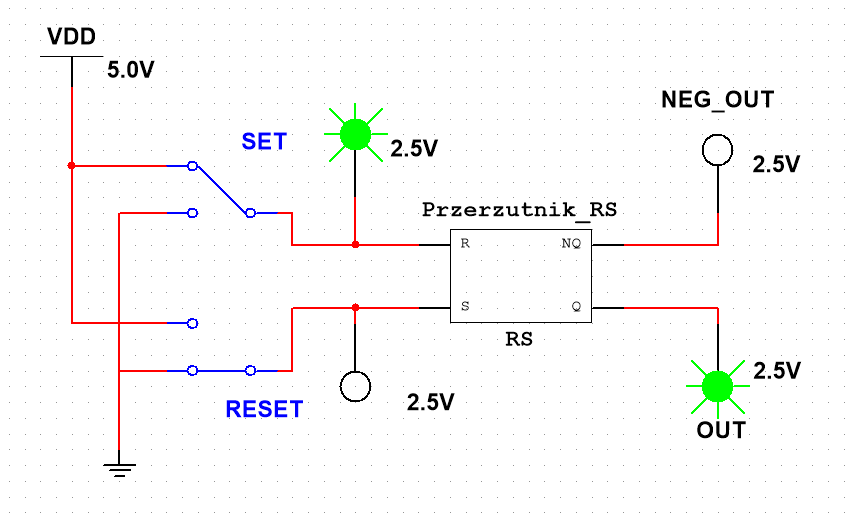
\includegraphics[width=0.8\textwidth]{images/2a_circuit_blackbox.png}
    \caption{Schemat idei rozwiązania}
    \label{rys:2a_circuit_blackbox}
\end{figure}

\begin{table}[h]
    \centering
    \begin{tabular}{|ccc|c|}
        \hline
        $S$ & $R$ & $Q$ & $Q_+$ \\
        \hline
        0   & 0   & 0   & 0     \\
        0   & 0   & 1   & 1     \\
        \hline
        0   & 1   & 0   & 0     \\
        0   & 1   & 1   & 0     \\
        \hline
        1   & 0   & 0   & 1     \\
        1   & 0   & 1   & 1    \\
        \hline
        1   & 1   & 0   & -     \\
        1   & 1   & 1   & -    \\
        \hline
    \end{tabular}
    \caption{Tabela prawdy przerzutnika RS}
    \label{tab:rs_truthtable}
\end{table}

Zauważmy, że w tabeli dla $S = R = 1$ brakuje wartości $Q_+$
Jest to tzw. stan zakazany, zatem zakładamy, że nie zachodzi i nie rozważamy
wyjścia bramki w takim przypadku.

\section{Rozwiązanie teoretyczne}

Szukamy funkcji logicznej określającej stan kolejnej iteracji $Q_+$ w zależności od stanu poprzedniego:
\begin{equation}
    Q_+ = Q_+(S, R, Q)
\end{equation}

W celu znalezienia tej funkcji posłużono się tabelą Karnough 
(pojawiają się w niej stany zabronione, jednak
są one niejako "poza dziedziną" funkcji, a
więc nie powinny nigdy zajść w prawidłowo użytkowanym przerzutniku):

\begin{figure}[H]
    \centering
    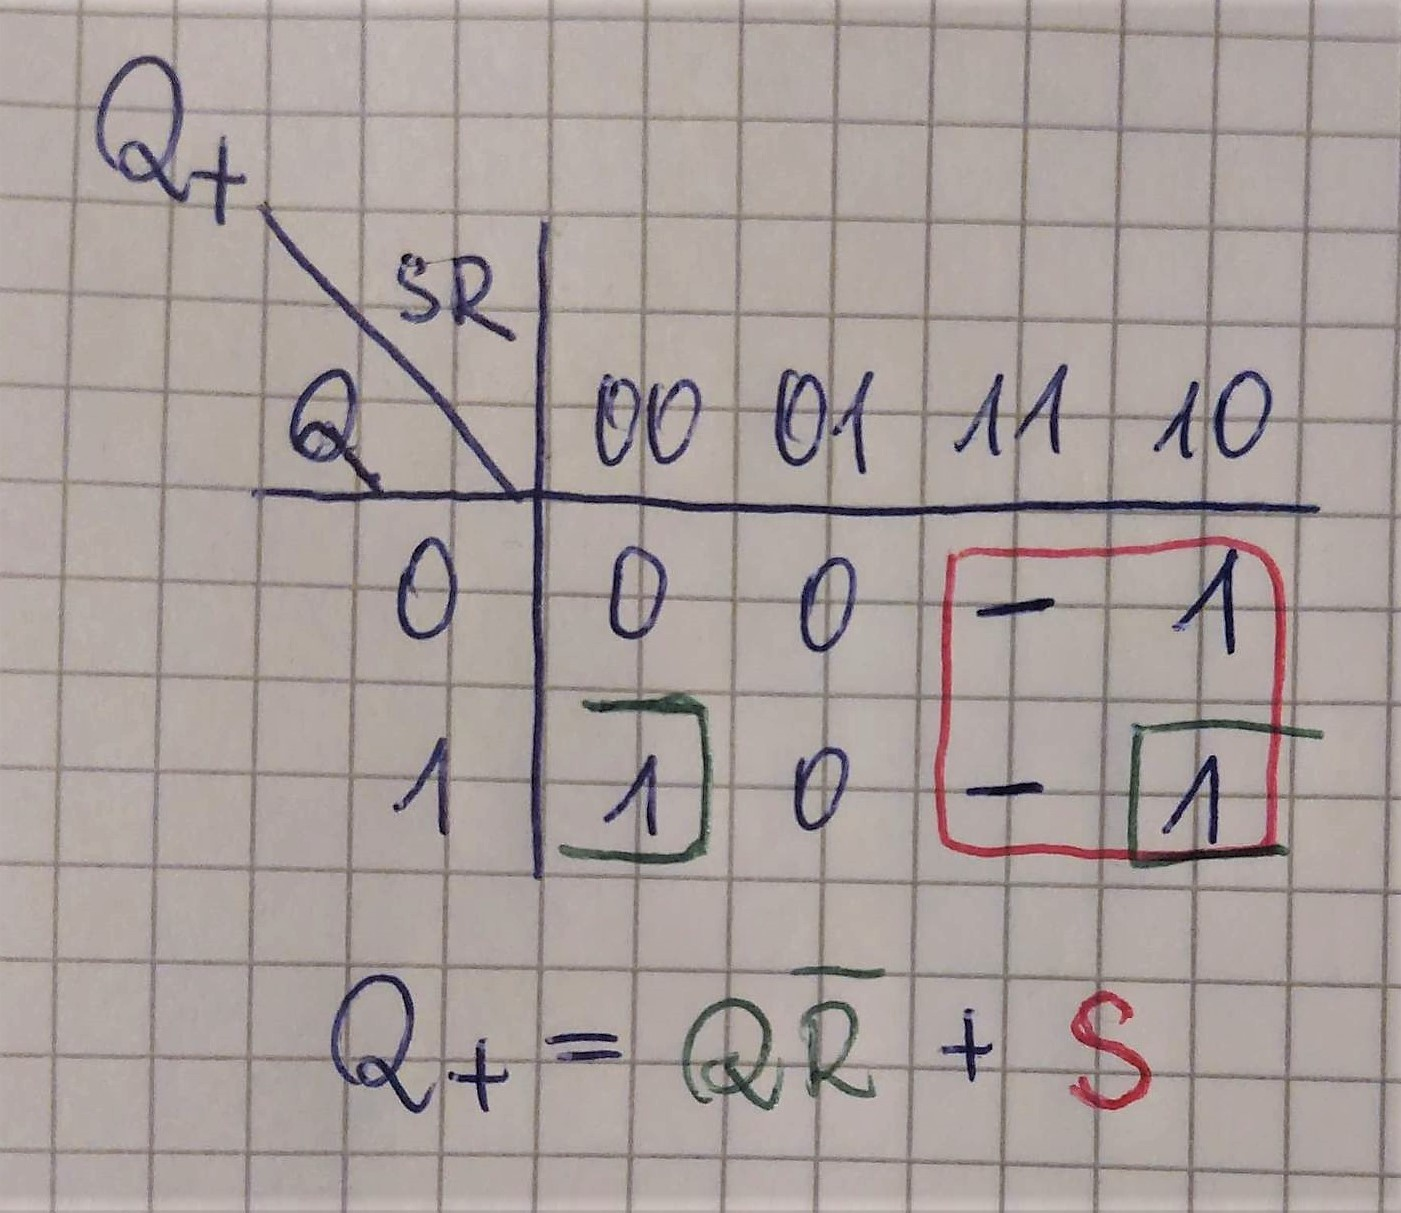
\includegraphics[width=0.3\linewidth]{images/rs_karnough.jpg}
    \caption{Tabela Karnough zastosowana w celu znalezienia funkcji logicznej przerzutnika RS}
    \label{fig:rs_karnough}
\end{figure}

Następnie przekształcono funkcję $Q_+$, aby zapisać ją przy pomocy funkcji NAND:

\begin{figure}[H]
    \centering
    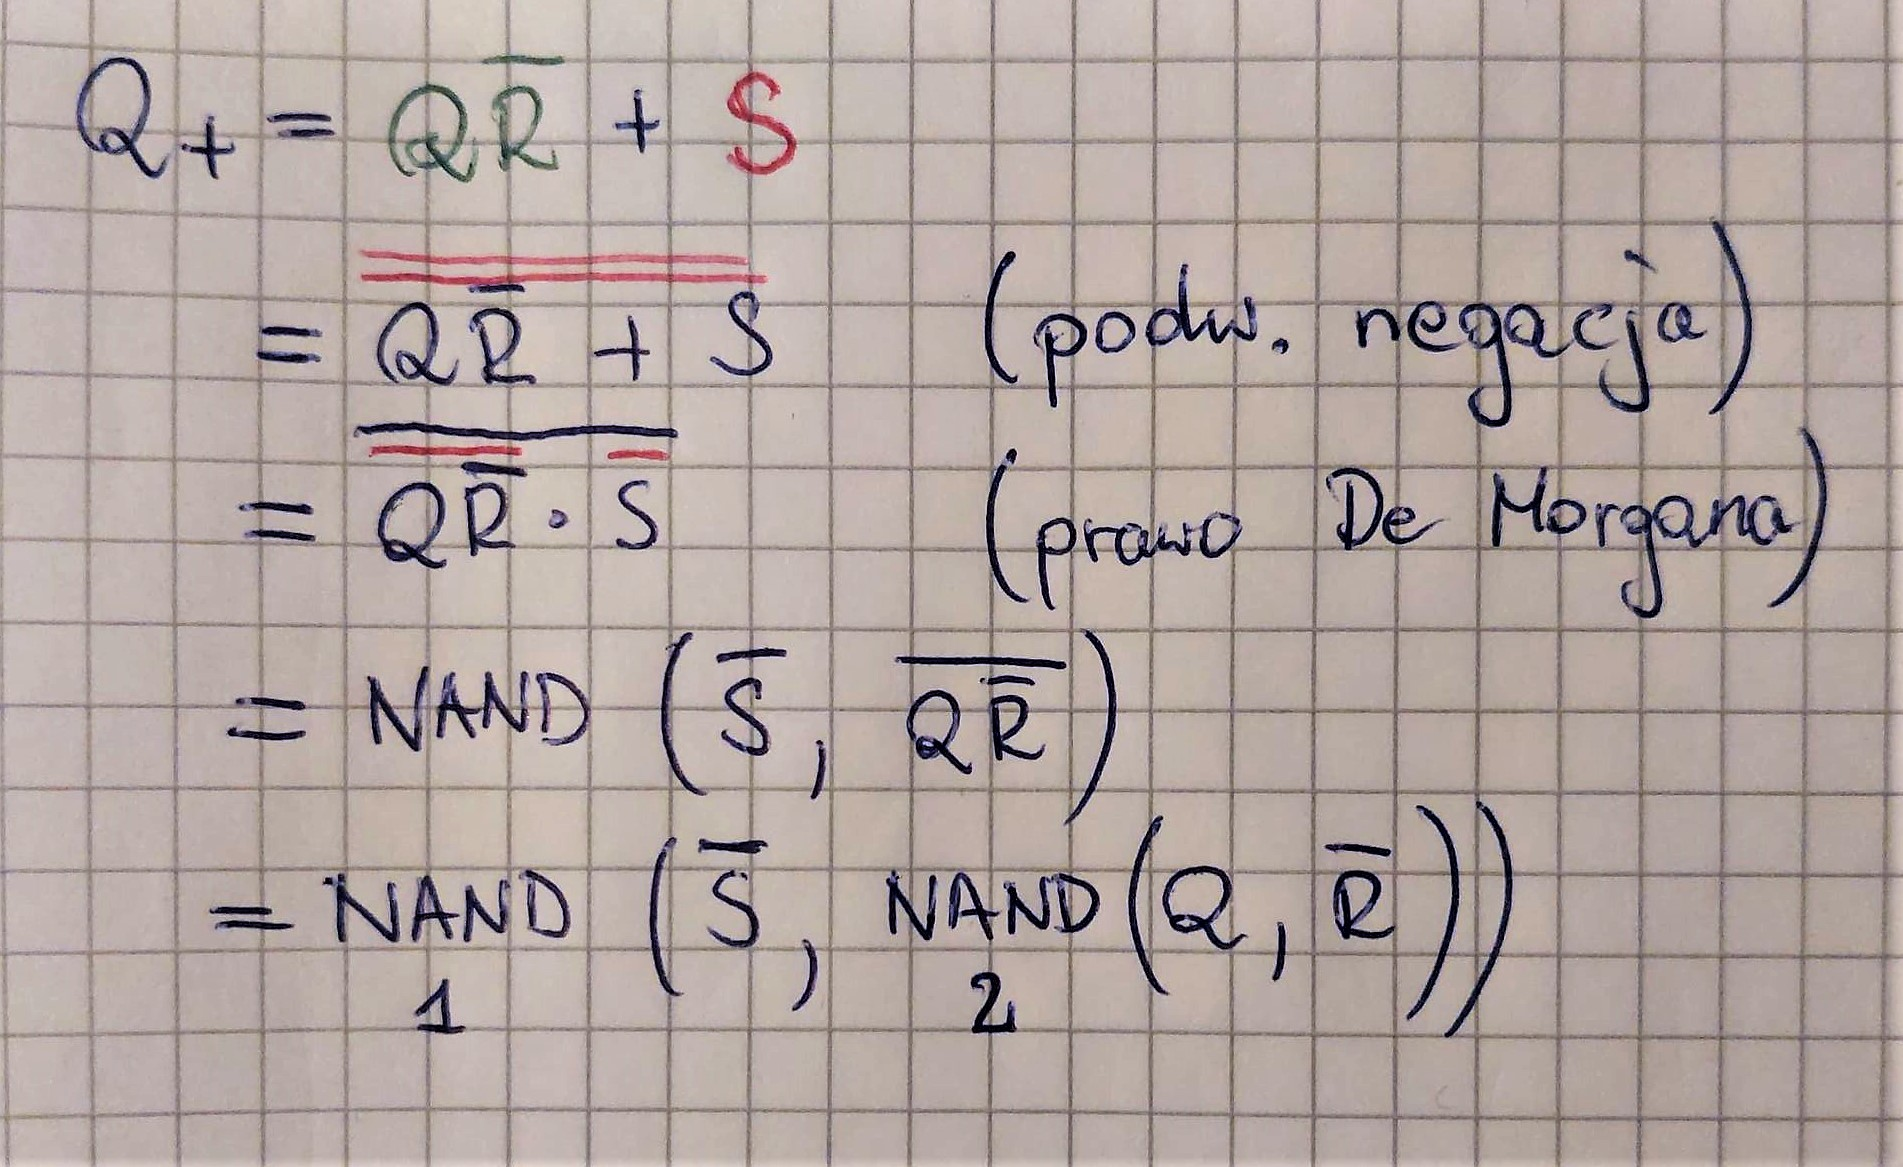
\includegraphics[width=0.6\linewidth]{images/rs_derivation.jpg}
    \caption{Przekształcenia wzoru funkcji logicznj do postaci złożonej z funkcji NAND}
    \label{fig:rs_derivation}
\end{figure}

Na podstawie wzoru funkcji sporządzono schemat układu, który został przedstawiony na poniższym rysunku:

\begin{figure}[H]
    \centering
    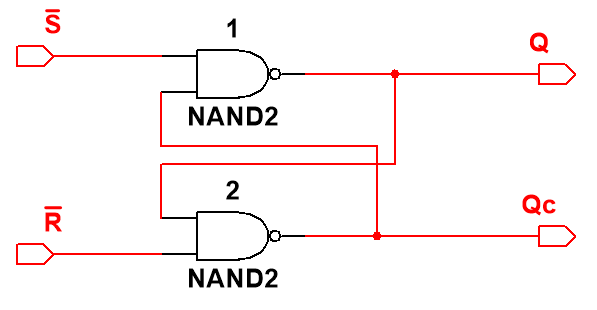
\includegraphics[width=0.5\linewidth]{images/rs_schematic.PNG}
    \caption{Schemat przerzutnika RS. Wejścia $\overline{S}$ i $\overline{R}$ są aktywne w stanie niskim.}
    \label{fig:rs_schematic}
\end{figure}

\section{Testy w programie Multisim}

Aby przetestować zaprojektowany układ, zbudowano następujący układ testowy w programie Multisim, 
który porównuje działanie układu z rzeczywistym przerzutnikiem RS:

\begin{figure}[H]
    \centering
    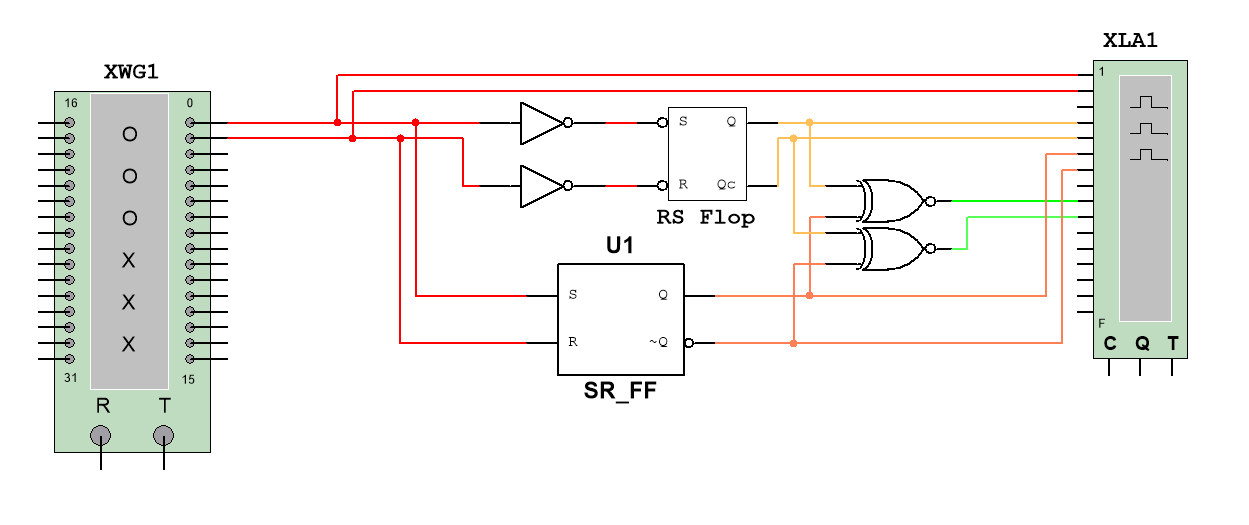
\includegraphics[width=0.9\linewidth]{images/rs_test.PNG}
    \caption{Schemat układu testowego.}
    \label{fig:rs_test}
\end{figure}

Generator słów bitowych ustawiono na następującą sekwencję, która testuje przejścia między wszystkimi
możliwymi stanami:

\begin{figure}[H]
    \centering
    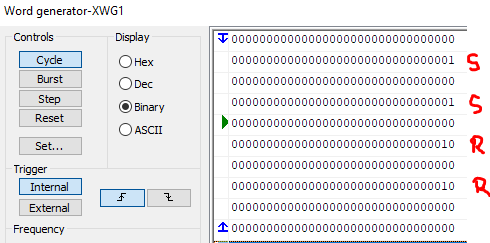
\includegraphics[width=0.6\linewidth]{images/rs_xwg.PNG}
    \caption{Sekwencja słów bitowych na wejściu układu testowego.}
    \label{fig:rs_xwg}
\end{figure}

Na analizatorze stanów logicznych zaobserwowano następujące dane:

\begin{figure}[H]
    \centering
    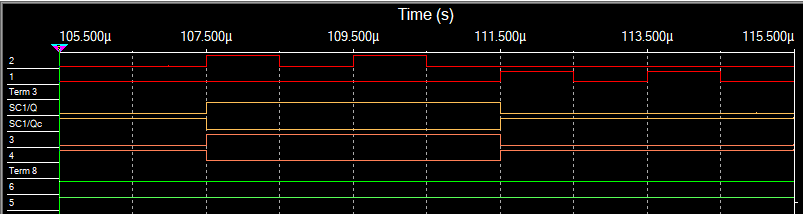
\includegraphics[width=0.8\linewidth]{images/rs_plot.PNG}
    \caption{Sekwencja słów bitowych na wejściu układu testowego.}
    \label{fig:rs_plot}
\end{figure}

Ciągły stan wysoki na wyjściach bramek XNOR sprawdzających równoważność układów dowodzi poprawności działania
przerzutnika.

\section{Wnioski}

\begin{enumerate}
    \item Przerzutnik RS jest prostym układem, który sprawdza się,
        gdy mamy pewność, że układ sterujący nim nie poda na wejściu stanu zabronionego $S = R = 1$. Jeśli przerzutnikiem
        steruje wprost użytkownik, lepiej zastosować przerzutnik JK, który jest odporny na niekontrolowane zachowanie.

    \item Synchronicznej wersji przerzutnika RS (takiej która zmienia stan 
    tylko podczas taktu zegara) można użyć do budowy rejestrów przesuwnych.
    
    \item Przerzutnik RS można zastosować w celu uniknięcia 
    "efektu skakania" przycisków i przełączników mechanicznych.

    \item Wszelkiego rodzaju detektory wartości krytycznej (zachodzenia danego zjawiska).
    Możemy podpiąć przerzutnik RS do detektora i jeśli zajdzie oczekiwane zjawisko,
    przerzutnik zostanie włącznony (SET. Wtedy nawet po dłuższym czasie będziemy
    w stanie stwierdzić czy zaszło dane zjawisko/warunek.
    Przykład: alarm przeciwpożarowy - przy wykryciu dymu, włączany jest 
    przerzutnik RS, który uruchamia syreny, bez możliwości automatycznego resetu.
    Zresetowanie jest możliwe tylko poprzez wciśniecie guzika (RESET), nie przez czujnik,
    który jest podłączony do wejścia SET.
\end{enumerate}

\chapter{Zadanie 2b}
Korzystając z wybranych przerzutników, proszę zbudować rejestr 
pierścieniowy. Rejestr ten powinien realizować dwie podstawowe 
funkcje wybierane przy pomocy 
pojedynczego przełącznika: ładowanie danych do rejestru i krążenie danych w rejestrze.

\section{Idea}

\begin{figure}[H]
    \centering
    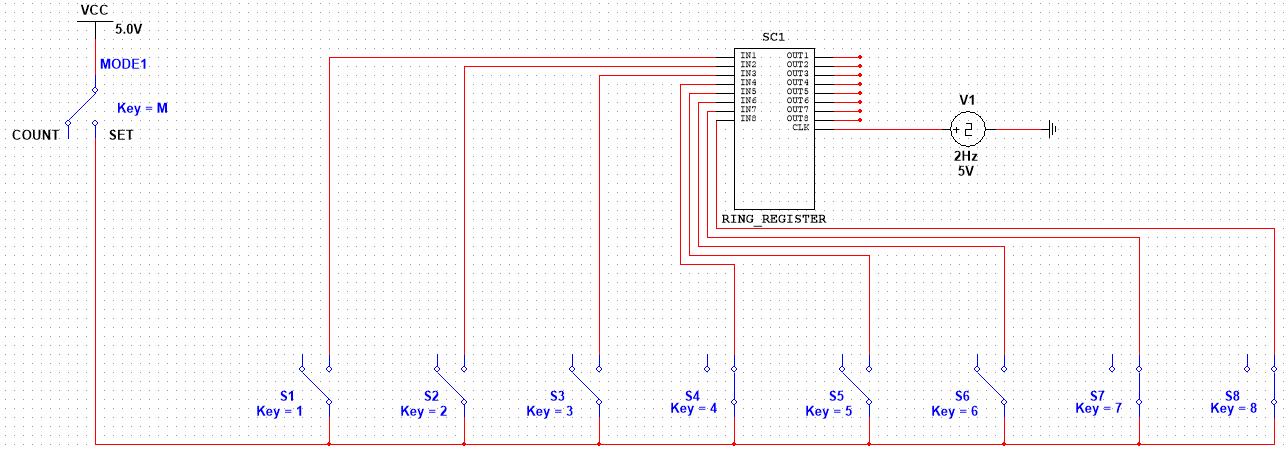
\includegraphics[width=0.8\linewidth]{images/2b_idea.png}
    \caption{Idea rozwiązania.}
    \label{fig:2b_idea}
\end{figure}

Przełącznik MODE
pozwala nam zmieniać tryb pracy na tryb ładowania lub 
krążenia danych. Przełączniki S1 do S8 pozwalają na ustawienie wartości poszczególnych
bitów rejestru kiedy przełącznik MODE jest w trybie SET.
Nasz rejestr będzie rejestr beðzie rejestrem PIPO (parallel in, parallel out).
Co oznacza, że może równolegle przejmować wejście i zwracać wyjście dla wszystkich
bitów przerzutnika.

\section{Wstęp teoretyczny}

Rejestr pierścieniowy to rejestr przesuwny, gdzie wyjście ostatniego przerzutnika
podłączone jest do wejścia przerzutnika pierwszego. W ten sposób wartości w rejestrze
mogą w ciągły sposób w nim krążyć. Do budowy rejestru użyliśmy 8 przerzutników $D$
w taki sposób, że wyjście poprzedniego połączone jest w wejściem kolejnego 
(jak w rejestrze przesuwnym). 


Na przykład, jeśli załadujemy do rejestru (w trybie SET) liczbę $10011111$, to
po przełączeniu w tryb COUNT wartości rejestru po kolejnych 8 taktach zegara przedstawia poniższa tabela.


\begin{table}[h!]
    \centering
    \begin{tabular}{|c|cccccccc|}
        \hline
        Czas & Q1 & Q2 & Q3 & Q4 & Q5 & Q6 & Q7 & Q8 \\
        \hline
        0 & 1 & 0 & 0 & 1 & 1 & 1 & 1 & 1 \\
        1 & 1 & 1 & 0 & 0 & 1 & 1 & 1 & 1 \\
        2 & 1 & 1 & 1 & 0 & 0 & 1 & 1 & 1 \\
        3 & 1 & 1 & 1 & 1 & 0 & 0 & 1 & 1 \\
        4 & 1 & 1 & 1 & 1 & 1 & 0 & 0 & 1 \\
        5 & 1 & 1 & 1 & 1 & 1 & 1 & 0 & 0 \\
        6 & 0 & 1 & 1 & 1 & 1 & 1 & 1 & 0 \\
        7 & 0 & 0 & 1 & 1 & 1 & 1 & 1 & 1 \\
        8 & 1 & 0 & 0 & 1 & 1 & 1 & 1 & 1 \\
        \hline
    \end{tabular}
    \caption{Stan bitów Q1 do Q8 rejestru pierścieniowego podczas przebiegu w czasie}
\end{table}

Jak widzimy po 8 taktach zegara (czyli liczbie równej długości rejestru) 
stan rejestru jest taki sam jak na początku - odbył się pełen cykl.


\section{Realizacja w Multisim}

\begin{figure}[H]
    \centering
    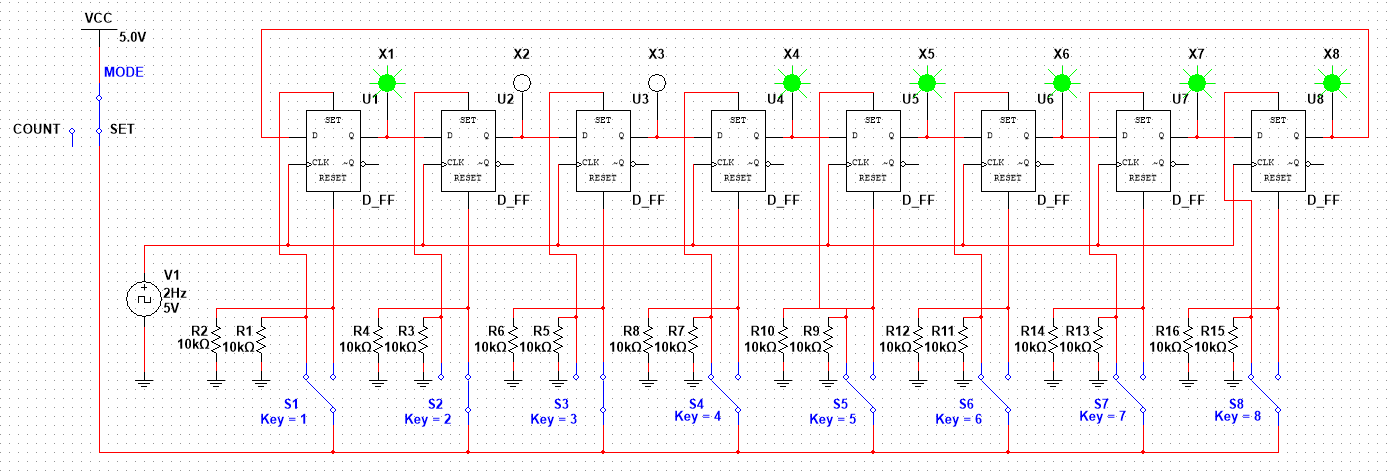
\includegraphics[width=1\textwidth]{images/2b_set_example.png}
    \caption{Układ w trybie SET, z przełącznikami ustawiajacymi wartość rejestru na 10011111}
    \label{rys:2b_set_example}
\end{figure}

\begin{figure}[H]
    \centering
    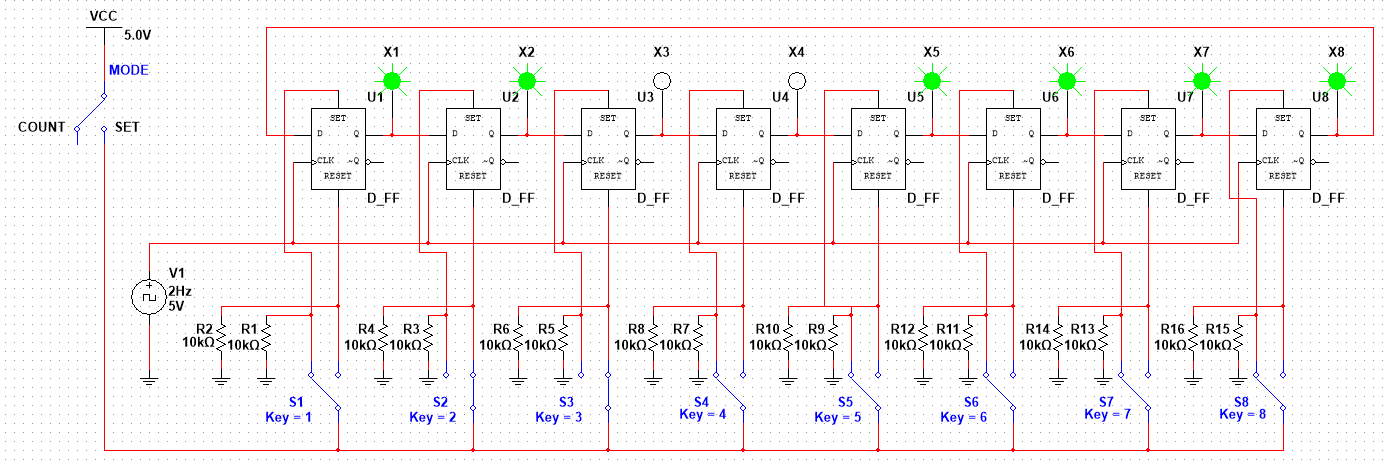
\includegraphics[width=1\textwidth]{images/2b_count_tick1_example.png}
    \caption{Układ w trybie COUNT po jednym takcie zegara}
    \label{rys:2b_count_tick1_example}
\end{figure}

\section{Testy}


Dla przetestowania układu stworzono podpukład CMP\_8BIT, czyli komparator liczb 8 bitowych, 
oparty na układzie N74F521N służący d porównywania liczb 8 bitowych.
Wyjście komparatora działa tak jak w N74F521N w trybie active-low a zatem 0 na wyjściu
oznacza równośc liczb.

\begin{figure}[H]
    \centering
    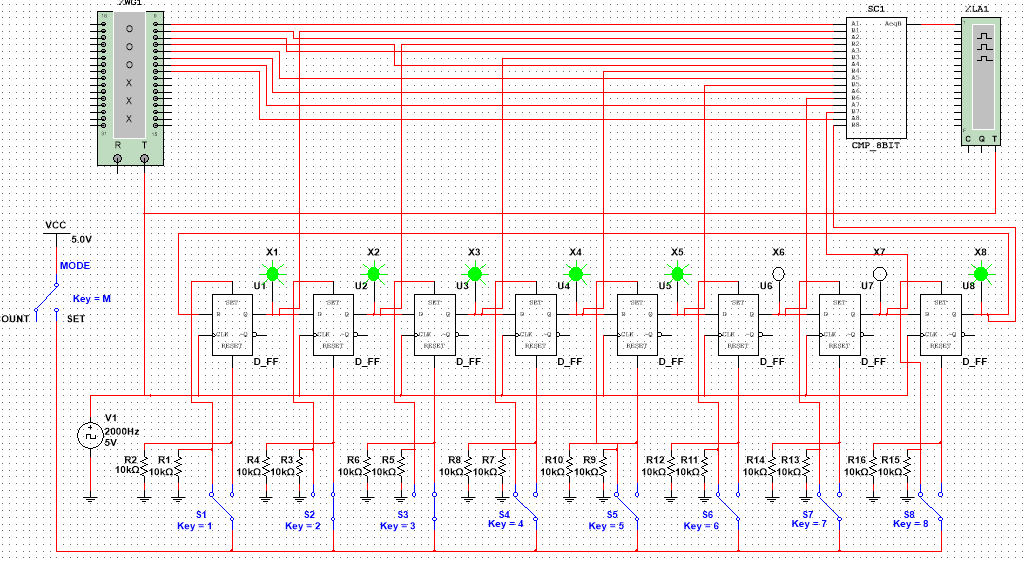
\includegraphics[width=1\textwidth]{images/2b_test_cir.png}
    \caption{Układ testowy}
    \label{rys:2b_test_cir}
\end{figure}

\begin{figure}[H]
    \centering
    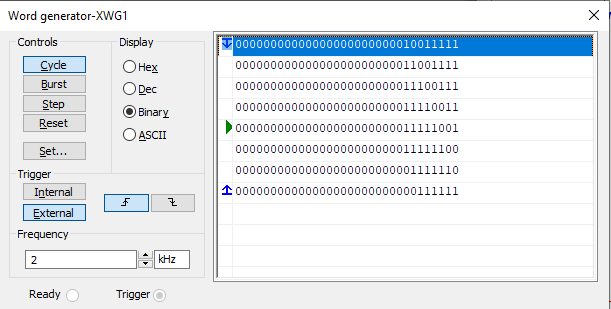
\includegraphics[width=1\textwidth]{images/2b_wg.png}
    \caption{Generator słów}
    \label{rys:2b_wg}
\end{figure}

\begin{figure}[H]
    \centering
    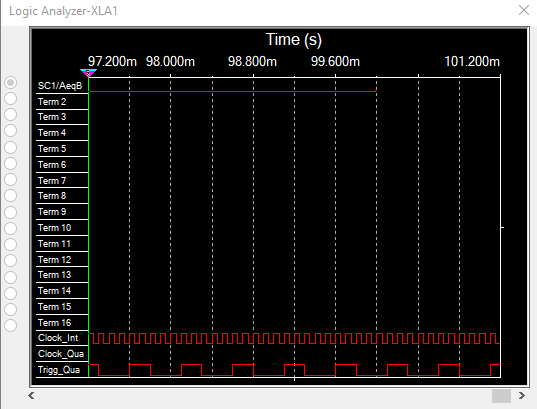
\includegraphics[width=1\textwidth]{images/2b_test_analyzer.png}
    \caption{Analizator logiczny pokazujacy wynik testu - ciągłe 0 - liczby równe podczas każdego taktu zegara}
    \label{rys:2b_test_analyzer}
\end{figure}

\section{Wnioski}

    \begin{enumerate}
        \item Używamy przerzutników D, które posiadają opcje ustawiania i resetowania. Bez tego, korzystając
        z "czystego" przerzutnika D nie moglibyśmy zrealizować funkcji ładowania danych do rejestru. 
        
        \item Nasz rejestr jest tzw. rejestrem PIPO (parallel in, parallel out), ale istnieją także wersje
        z wejściem i wyjściem szeregowym SIPO, PISO i SISO. Każdy z nich znajduje zastosowania w nieco innych 
        przypadkach, u nas konieczne było zastosowanie wejścia równoległego do realizacji funkcji ładowania, a 
        równoległe wyjście pozwala na efektywne testowanie.

        \item Rejestru pierścieniowego można użyć do konstrukcji lampek choinkowych, które cyklicznie zmieniają
        się zgodnie z bitami krążącymi w rejestrze. Przesunięcia rejestru tworzą iluzję animacji na choince.
        
    \end{enumerate}

\end{document}
